La gestion de la documentation a initialement été mise en place sous la forme d'un wiki sur le dépôt github du projet \href{https://github.com/gromax/uPSimulator/wiki}{uPSimulator: Simulateur de processeur} (\url{https://github.com/gromax/uPSimulator/wiki})

Dans un second temps, le choix s'est porté sur \href{https://www.sphinx-doc.org/en/master/index.html}{Sphinx} qui permet de renseigner directement le code source, d'exporter dans de multiples formats et d'inclure des fragments exemples.


\begin{figure}[h!]
	\centering
	\begin{subfigure}[b]{0.43\textwidth}
		\inputminted[firstline=0,lastline=43,frame = single, fontsize=\scriptsize, tabsize=2, breaklines, autogobble]{python}{litteral.py}
		\caption{Code commenté}
	\end{subfigure}
\hfill
	\begin{subfigure}[b]{0.475\textwidth}
	\frame{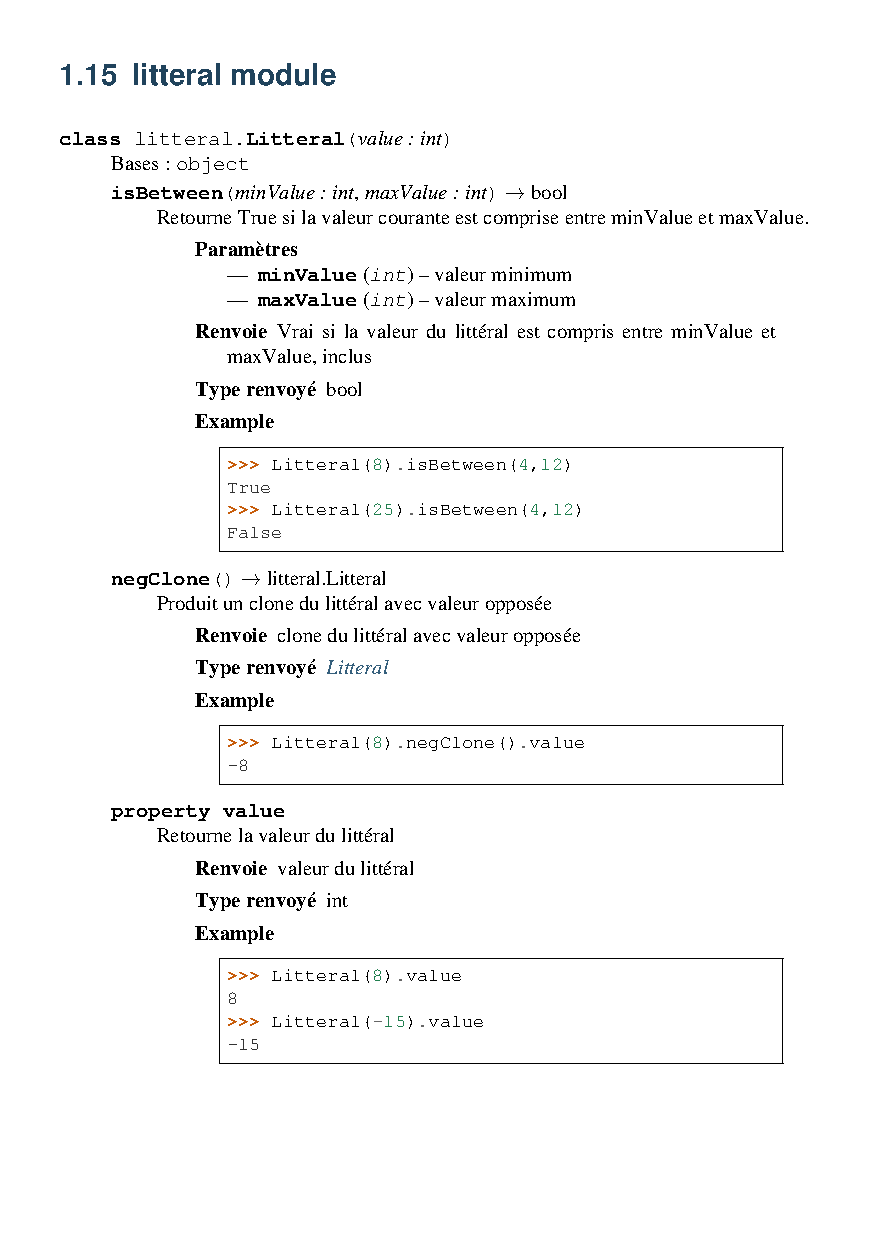
\includegraphics[width=\textwidth]{Pictures/SphinxDocExemple}}
	\caption{Documentation compilée}
	\end{subfigure}
	\caption{Extrait de documentation Sphinx}
	\label{fig:sphinxdocexemple}
\end{figure}